\chapter{Review of Previous Work}
\label{sec:lit_review} % Always give a unique label
% use \chaptermark{}
% to alter or adjust the chapter heading in the running head

% \section{Literature Review}
% \label{sec:InterventionRobotics}

\section{Needle Geometry}
Beveled-tip needles deflect during insertion due to asymmetric cutting force at the needle tip. The cutting forces on the tip of the needle, shown in Figure \ref{fig:tip_forces} can be modeled as a point load with transverse  and radial components relative to the needle shaft\cite{misra_mechanics_2010}. Friction and damping force are transverse forces distributed along the needle shaft, while pushback from deformed tissue is a distributed radial force. Figure \ref{fig:needle_forces} shows the point and distributed loads on the needle shaft.

\begin{figure}[h]
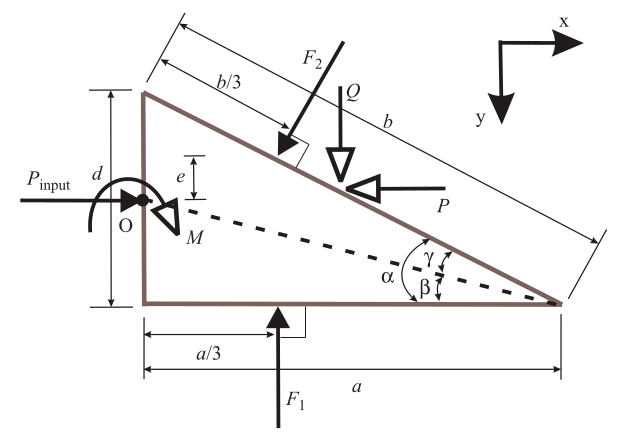
\includegraphics[width=1.0\textwidth]{Fig/chap2/misra_tip_forces.png}
\caption{Free-body diagram depicting forces acting on the needle tip during insertion into an elastic medium (from Misra, 2010\cite{misra_mechanics_2010}).}
\label{fig:tip_forces}
\end{figure}

\begin{figure}[h]
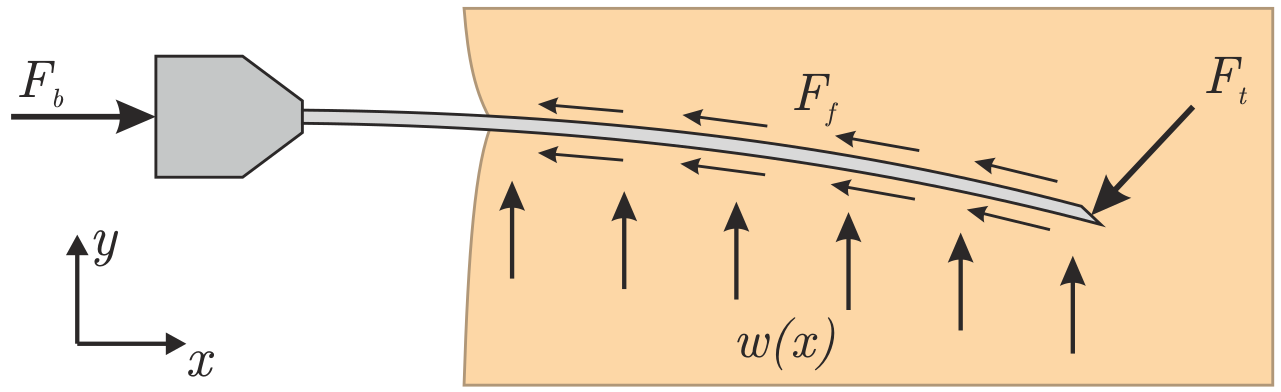
\includegraphics[width=1.0\textwidth]{Fig/chap2/roesthius_needle_forces.png}
\caption{Point and distributed forces acting on the needle during insertion (from Roesthuis, 2012\cite{roesthuis_mechanics-based_2012}).}
\label{fig:needle_forces}
\end{figure}

\section{Needle Modeling}
The goal of research in this area is to produce a model of needle behavior that accurately predicts the motion of the needle tip during insertion so that a needle trajectory can be planned and accurately followed even when few or no needle tip observations can be made.

\subsection{Non-Holonomic Kinematics}
The non-holonomic kinematics of a beveled-tip needle can be represented by modeling the needle as a bicycle with the front wheel fixed at a constant steering angle\cite{webster_nonholonomic_2006,cowan_robotic_2011}. This model is illustrated in figure \ref{fig:webster_nonholonomic_model}. Since the steering angle is determined by the shape of the needle, the stiffness of the tissue, and the velocity of insertion, steering angles must be calculated for individual insertions. 

\begin{figure}[h]
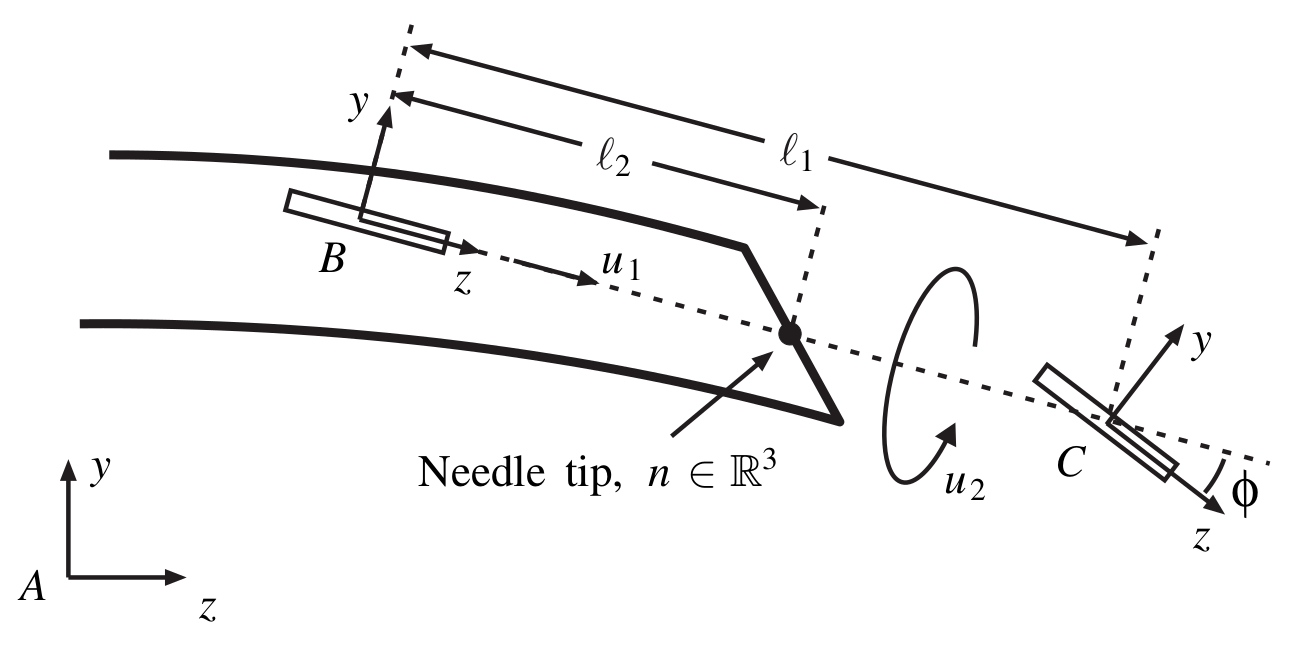
\includegraphics[width=1.0\textwidth]{Fig/chap2/webster_nonholonomic_model.png}
\caption{Nonholonomic model in which the needle tip is represented as a bicycle with a fixed front-wheel steering angle (from Webster, 2006\cite{webster_nonholonomic_2006}).}
\label{fig:webster_nonholonomic_model}
\end{figure}

Subsequent work accounts for forces on the needle that cannot be modeled as components of the steering angle, such as dynamic friction and torsion in the needle shaft\cite{reed_modeling_2009, swensen_torsional_2014}. These works still assume a constant steering angle, which implies that the needle is inserted into a homogeneous material. This assumption does not apply for most insertions into tissue, limiting the utility of the nonholonomic model for clinical applications.

\subsection{Finite Element Models}
Finite Element (FE) modeling of the needle and surrounding medium addresses some of the drawbacks of the kinematic needle model, such as the ability to model inconsistent deflection when inserting through nonhomogeneous tissue\cite{goksel_modeling_2009}. FEM-based approaches use several types of finite elements, including angular springs and beam elements. While the problem is often simplified as a 2D mesh in a plane, the approach is extensible to 3D\cite{chentanez_interactive_2009}.

FE modeling necessitates explicit representations for the sliding interface between the needle shaft and the surrounding tissue and for the elastic mechanical properties that govern the deformation of tissue during insertion\cite{dehghan_comparison_2006}. Since needles are very slender and the magnitude of deflection is comparatively large, the assumption of linear displacement usually used during FE analysis is not applicable and a computationally-intensive numerical solver is required to solve for nonlinear displacement.



\begin{figure}[h]

\includegraphics[width=1.0\textwidth]{Fig/placeholder.png}
\caption{Finite element model which represents the needle as a series of angular springs interacting with a 2D mesh\cite{goksel_modeling_2009}.}
\label{fig:needle_fe_model}
\end{figure}

\subsection{Mechanical Models}
Other works model the needle as an Euler-Bernoulli beam, with the forces acting on the needle divided into a force acting on the needle tip and a distributed load acting on the needle shaft. The tip force is related to the force required to cut through the tissue, which depends on the insertion velocity\cite{barnett_fracture_2015}. The distributed shaft load is related to the stiffness and viscous coefficient of the tissue\cite{abayazid_integrating_2013}.

Another approach is to represent the shape of the needle as a polynomial and use mechanical bending energy to choose the polynomial coefficients\cite{roesthuis_modeling_2015,misra_mechanics_2010,abayazid_integrating_2013}. This accounts for needle deflection and deformation of surrounding tissue, which allows calculation of the force on the needle base.

Mechanical models require direct measurement of the elastic modulus, stiffness, and cutting force of the tissue and the elastic modulus of the needle. The tissue is generally assumed to be homogeneous for simplicity.

\begin{figure}[h]
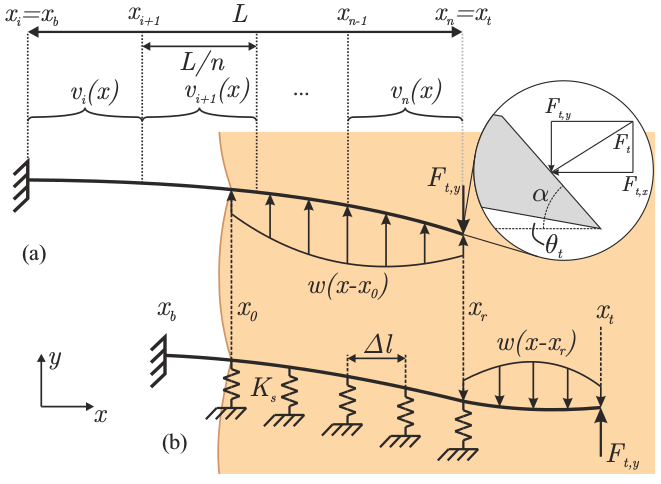
\includegraphics[width=1.0\textwidth]{Fig/chap2/roesthuis_two_bend_beam.png}
\caption{Mechanical model of a needle in a two-bend configuration (from Roesthuis, 2012\cite{roesthuis_mechanics-based_2012}).}
\label{fig:needle_mech_model}
\end{figure}

\section{Needle Steering}

The different approaches to needle steering can be generalized as minimally-invasive methods to guide a needle to a desired point in the body using control inputs applied outside the body. The various methods produced in this line of research can be placed along a spectrum of mechanical complexity at the needle tip, ranging from methods for steering a needle using only control inputs at its base, to needles with some actuation at the tip and along the shaft, to continuum robots. 

Needle steering strategies rely on the asymmetric force at the tip of a beveled needle as a control input to direct the needle along a desired trajectory. Rotating the needle tip changes the direction of the force vector, allowing the direction of deflection to be controlled. Steering algorithms that take advantage of this behavior include duty cycle steering, CURV steering, and continuous-rotation steering.

Symmetric-tip needles are not subject to significant asymmetric tip for during insertion\cite{dimaio_needle_2003}. While the magnitude of deflection during insertion is reduced, the direction of deflection is inconsistent, so symmetric-tipped needles cannot be steered by rotating the needle tip. An alternative strategy steers the needle by moving its base outside the tissue, which induces a bend in the needle shaft\cite{glozman_image-guided_2007}.

Curved- or kinked-tip needles use similar mechanical principles to steer as beveled-tip needles, but the addition of a pre-bent section greatly increases the asymmetric force applied to the needle tip during insertion\cite{reed_integrated_2008}. This allows the needle to achieve a tighter turning radius, especially if the needle shaft is made of nitinol wire. Kinked-tip needles cause more tissue damage than beveled-tip needles when steered using a rotation-based strategy, but needles with passively-actuated tips have been developed to mitigate this by straightening during continuous rotation\cite{swaney_flexure-based_2013}. Needles with fully-actuated tips can be steered along a trajectory without rotating the needle\cite{roesthuis_modeling_2015}. A disadvantage of curved-tip needles is that the tip translates during rotation, which violates the assumption of the nonholonomic kinematic model that the needle will only move along the tip vector\cite{reed_integrated_2008}.

\begin{figure}[h]

\includegraphics[width=1.0\textwidth]{Fig/placeholder.png}
\caption{Example of a needle with a pre-curved tip\cite{reed_integrated_2008}.}
\label{fig:kinked_tip}
\end{figure}

\begin{figure}[h]
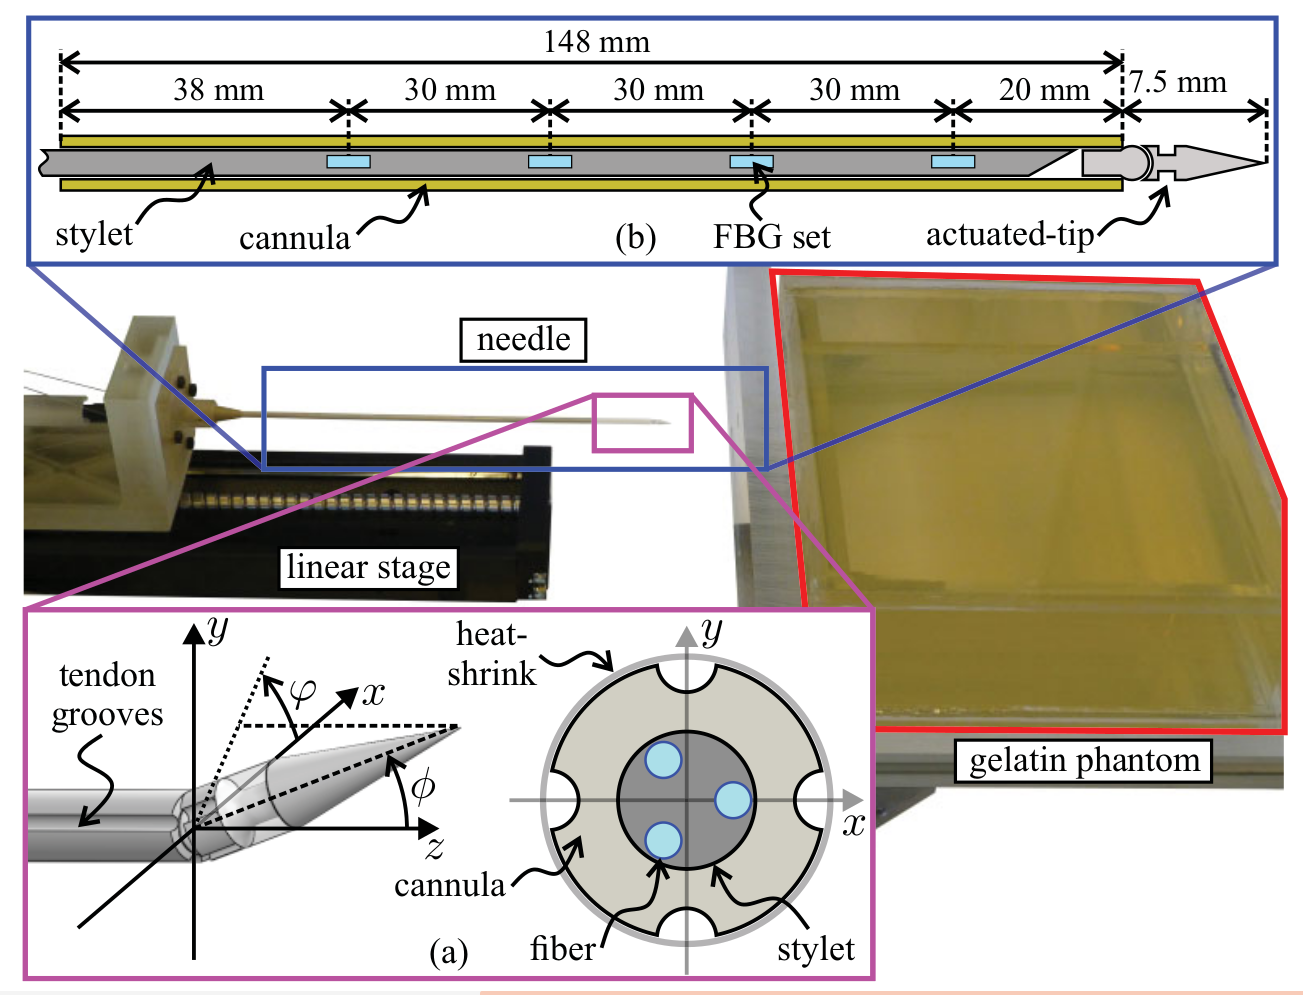
\includegraphics[width=1.0\textwidth]{Fig/chap2/actuated_tip_needle.png}
\caption{Custom-manufactured steerable needle with an actuated tip and Fiber Bragg Grating strain gauges(from Roesthuis, 2015\cite{roesthuis_modeling_2015}).}
\label{fig:actuated_tip}
\end{figure}

Concentric-tube needles consist of several nested pre-bent tubes\cite{webster_mechanics_2009, rucker_geometrically_2010, dupont_design_2010-1}. An example with three concentric segments is shown in Figure \ref{fig:concentric_tubes}. The needle can be actively curved or straightened by rotating the tubes so their directions of curvature are aligned or in opposition. These needles experience potentially-undesired releases of energy when the concentric elements snap between equilibrium states.

- Problems with these approaches, and with approaches that use custom needles in general, is that there aren't any clinically-available biopsy needles of these types. Need to be able to steer straight beveled-tip needles if we want to use what's out there right now.

- Potential for tissue damage along insertion trajectory is risky.

\begin{figure}[h]
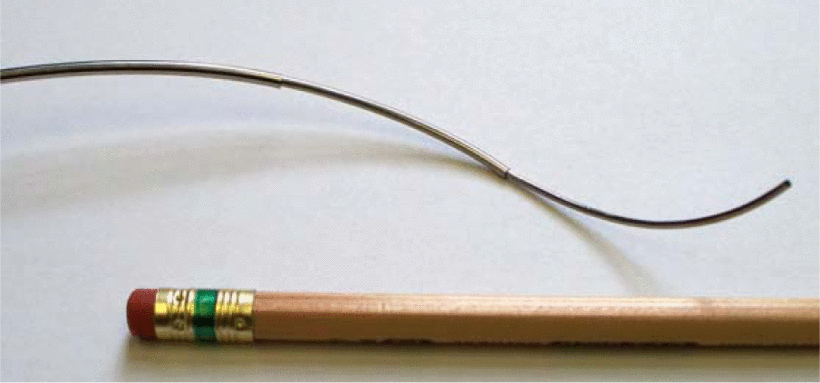
\includegraphics[width=1.0\textwidth]{Fig/chap2/concentric_needle.png}
\caption{Example of a steerable concentric-tube needle with three concentric segments (from Rucker, 2010\cite{rucker_geometrically_2010}).}
\label{fig:concentric_tubes}
\end{figure}

\section{Needle Localization}
Existing work in needle localization generally operates on individual scans or video frames in isolation. It would be very useful to use the results from processing a previous image to find the needle in the current image. Adding the change in the forward kinematics of the needle would improve this process as well.

\subsection{Coronal and Sagittal Plane Imaging}
Prior work by our research group demonstrated closed-loop MR imaging in the coronal and sagittal planes to follow the needle during insertion\cite{patel_closed-loop_2015}. As shown in Figure \ref{fig:patel_mri_tracking}, the needle tip is captured in each scan and its measured position of the centroid of the tip artifact is used to plan the pose of the subsequent scan in the perpendicular plane. The field of view of each plane is sized based on the maximum anticipated deflection of the needle between scans.

\begin{figure}[h]
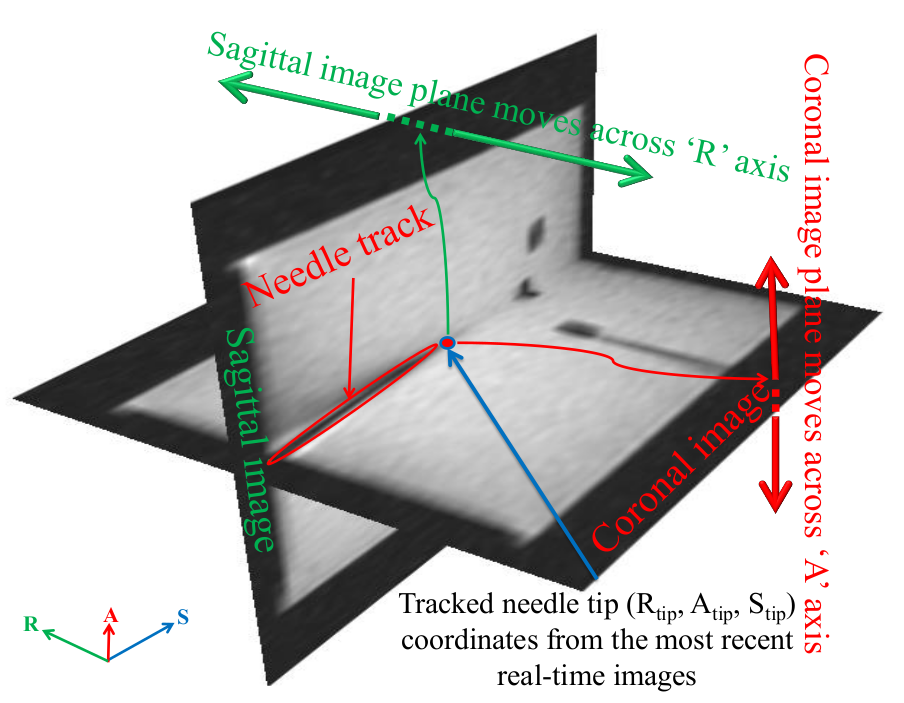
\includegraphics[width=1.0\textwidth]{Fig/chap2/patel_mri_tracking.png}
\caption{Alternating-planes strategy to track the needle tip during insertion (from Patel, 2015\cite{patel_closed-loop_2015}).}
\label{fig:patel_mri_tracking}
\end{figure}

A major risk with this approach is the loss of tracking if the needle tip is not found in one of the scans because the key piece of information used to plan the position of each scan is the location of the needle tip in the immediately-previous scan. Since the scan planes are parallel to the needle shaft and could only be several millimeters thick, a small error in the placement of one scan plane could result in failure to capture the need.e This risk can be mitigated by making the thickness of the scan planes sufficient to capture the needle tip even if it deflects significantly between scans. However, high scan plane thickness reduces the clarity of features in MR images, which would be detrimental for identifying anatomical features near the needle.


\subsection{Transverse Plane Imaging}
Imaging in the plane normal to the needle shaft captures the needle in cross-section. This avoids the problem of imaging in a plane that does not contain the needle, but it is more challenging to find the plane containing the needle tip. For US scanning\cite{carriere_needle_2015,rossa_adaptive_2016,vrooijink_needle_2014}, the transducer can be mounted on a motorized platform and moved in synchronization with the needle base to capture the same point on the needle in cross-section throughout insertion, as shown in Figure \ref{fig:transverse_planes_us}.

\begin{figure}[h]
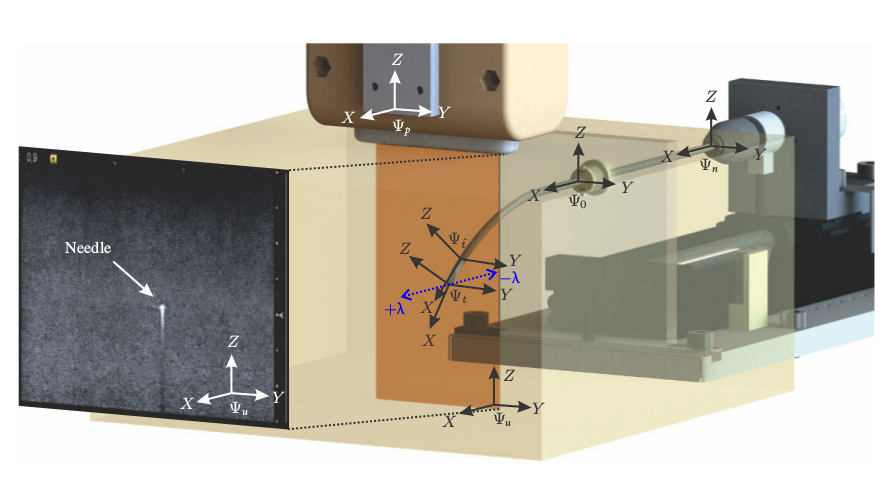
\includegraphics[width=1.0\textwidth]{Fig/chap2/vrooijink_US_tracking.png}
\caption{Needle tracking in US via imaging in the transverse plane (from Vrooijink, 2014\cite{vrooijink_needle_2014}).}
\label{fig:transverse_planes_us}
\end{figure}

\subsection{3D Imaging}
NeedleFinder is a 3D Slicer extension for needle localization and segmentation\cite{pernelle_validation_2013}. Figure \ref{fig:needlefinder} shows several catheters automatically segmented using NeedleFinder. Given a manually-selected tip position, NeedleFinder searches through sequential axial scan planes and finds the cross-sections of the artifacts or voids in each layer. An angular-spring finite element model defined by the shape and stiffness of the needle is fit to the detected needle points. Manual selection of each needle tip is required because of the difficulty of automatically distinguishing each needle from anatomical features and noise in the MR images.

\begin{figure}[h]
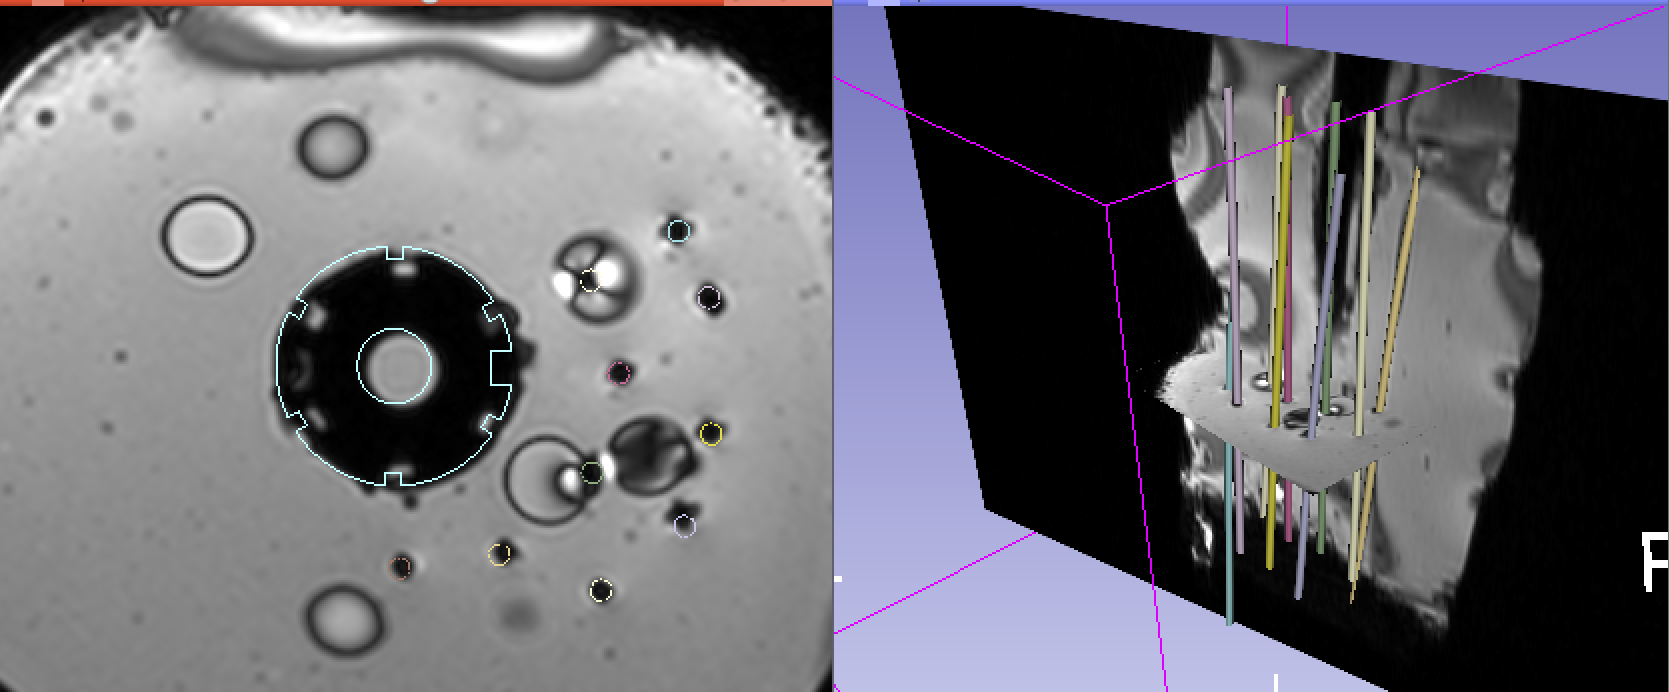
\includegraphics[width=1.0\textwidth]{Fig/chap2/needlefinder.png}
\caption{Catheters semi-automatically segmented in 3D MRI data using the NeedleFinder Slicer extension (from Pernelle, 2013\cite{pernelle_validation_2013}).}
\label{fig:needlefinder}
\end{figure}

Other research models susceptibility artifact shapes for metal fiducial markers in MR data to automatically segment the markers and determine their poses\cite{zijlstra_fast_2017}. This approach could probably be extended to detect needle tip poses from tip artifacts with greater precision than thresholding by intensity, but the variation in the needle artifact with the orientation of the needle relative to the direction of the magnetic field would present some challenges.

In both US and MR images, the time required to resolve a 3D volume is higher than for a 2D plane, so 3D imaging is generally not suitable for real-time tracking or control.

\subsection{Non-Imaging Techniques}
An alternative method for detecting the position and shape of the needle is to add sensors to the needle to directly measure its deflection. One approach, shown in Figure \ref{fig:needle_fbg} is to embed Fiber Bragg Grating optical sensors into the shaft of the needle\cite{roesthuis_three-dimensional_2014}. These sensors measure the strain in the needle as it bends and allow the shape of the needle to be calculated throughout insertion to achieve robotic steering. This approach requires specially-modified needles, precluding the use of common clinical-style biopsy needles.

\begin{figure}[h]
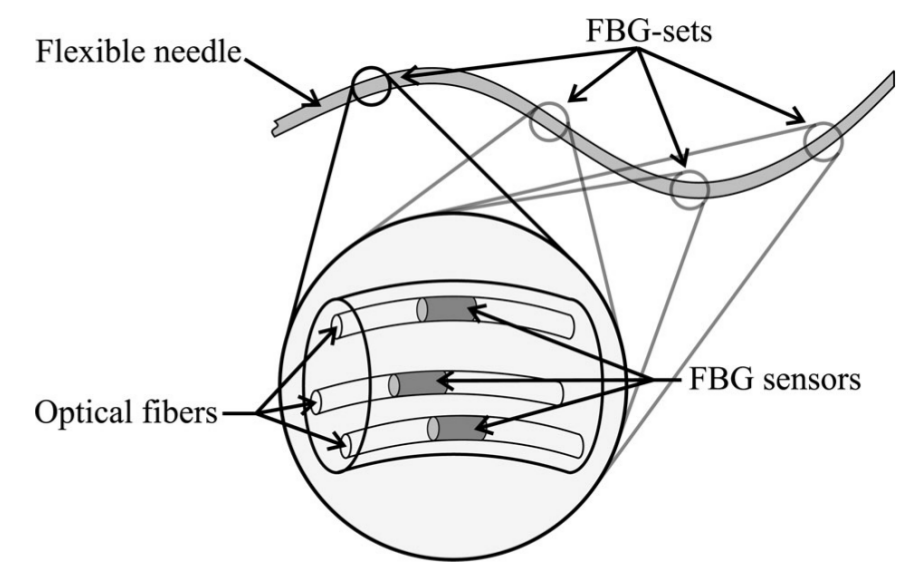
\includegraphics[width=1.0\textwidth]{Fig/chap2/fbg_needle.png}
\caption{Placement of Fiber Bragg Grating sensors on a specially-modified needle (from Roesthuis, 2014\cite{roesthuis_three-dimensional_2014}).}
\label{fig:needle_fbg}
\end{figure}

Another option is to attach magnetic tracking coils to the needle shaft and use an external sensor unit like the Polaris to measure their 6-DOF poses and compute the needle shape.
\cite{patil_needle_2014,wang_real-time_2015} This isn’t compatible with the MRI environment.
